% Options for packages loaded elsewhere
\PassOptionsToPackage{unicode}{hyperref}
\PassOptionsToPackage{hyphens}{url}
\PassOptionsToPackage{dvipsnames,svgnames*,x11names*}{xcolor}
%
\documentclass[
  11pt,
]{article}
\usepackage{amsmath,amssymb}
\usepackage{lmodern}
\usepackage{ifxetex,ifluatex}
\ifnum 0\ifxetex 1\fi\ifluatex 1\fi=0 % if pdftex
  \usepackage[T1]{fontenc}
  \usepackage[utf8]{inputenc}
  \usepackage{textcomp} % provide euro and other symbols
\else % if luatex or xetex
  \usepackage{unicode-math}
  \defaultfontfeatures{Scale=MatchLowercase}
  \defaultfontfeatures[\rmfamily]{Ligatures=TeX,Scale=1}
\fi
% Use upquote if available, for straight quotes in verbatim environments
\IfFileExists{upquote.sty}{\usepackage{upquote}}{}
\IfFileExists{microtype.sty}{% use microtype if available
  \usepackage[]{microtype}
  \UseMicrotypeSet[protrusion]{basicmath} % disable protrusion for tt fonts
}{}
\makeatletter
\@ifundefined{KOMAClassName}{% if non-KOMA class
  \IfFileExists{parskip.sty}{%
    \usepackage{parskip}
  }{% else
    \setlength{\parindent}{0pt}
    \setlength{\parskip}{6pt plus 2pt minus 1pt}}
}{% if KOMA class
  \KOMAoptions{parskip=half}}
\makeatother
\usepackage{xcolor}
\IfFileExists{xurl.sty}{\usepackage{xurl}}{} % add URL line breaks if available
\IfFileExists{bookmark.sty}{\usepackage{bookmark}}{\usepackage{hyperref}}
\hypersetup{
  colorlinks=true,
  linkcolor=Maroon,
  filecolor=Maroon,
  citecolor=Blue,
  urlcolor=blue,
  pdfcreator={LaTeX via pandoc}}
\urlstyle{same} % disable monospaced font for URLs
\usepackage[margin=1in]{geometry}
\usepackage{graphicx}
\makeatletter
\def\maxwidth{\ifdim\Gin@nat@width>\linewidth\linewidth\else\Gin@nat@width\fi}
\def\maxheight{\ifdim\Gin@nat@height>\textheight\textheight\else\Gin@nat@height\fi}
\makeatother
% Scale images if necessary, so that they will not overflow the page
% margins by default, and it is still possible to overwrite the defaults
% using explicit options in \includegraphics[width, height, ...]{}
\setkeys{Gin}{width=\maxwidth,height=\maxheight,keepaspectratio}
% Set default figure placement to htbp
\makeatletter
\def\fps@figure{htbp}
\makeatother
\setlength{\emergencystretch}{3em} % prevent overfull lines
\providecommand{\tightlist}{%
  \setlength{\itemsep}{0pt}\setlength{\parskip}{0pt}}
\setcounter{secnumdepth}{-\maxdimen} % remove section numbering
\usepackage{setspace}
\usepackage{float}
\usepackage{mathtools}
\usepackage{natbib}
\usepackage[linesnumbered,ruled,vlined]{algorithm2e}
\setcitestyle{numbers,square,comma}
\usepackage{verbatim}
\usepackage{amsthm}
\usepackage{comment}
\ifluatex
  \usepackage{selnolig}  % disable illegal ligatures
\fi
\usepackage[]{natbib}
\bibliographystyle{plainnat}

\title{Semi-Parametric Manifold Clustering}
\author{}
\date{\vspace{-2.5em}}

\begin{document}
\maketitle

\newcommand{\diag}{\mathrm{diag}}
\newcommand{\tr}{\mathrm{Tr}}
\newcommand{\blockdiag}{\mathrm{blockdiag}}
\newcommand{\indep}{\stackrel{\mathrm{ind}}{\sim}}
\newcommand{\iid}{\stackrel{\mathrm{iid}}{\sim}}
\newcommand{\Bernoulli}{\mathrm{Bernoulli}}
\newcommand{\Betadist}{\mathrm{Beta}}
\newcommand{\Uniform}{\mathrm{Uniform}}
\newcommand{\BG}{\mathrm{BernoulliGraph}}
\newcommand{\Categorical}{\mathrm{Categorical}}
\newcommand{\Multinomial}{\mathrm{Multinomial}}
\newcommand{\RDPG}{\mathrm{RDPG}}
\newcommand{\GRDPG}{\mathrm{GRDPG}}
\newtheorem{definition}{Definition}
\newtheorem{theorem}{Theorem}
\newtheorem{lemma}{Lemma}
\theoremstyle{remark}
\newtheorem*{remark}{Remark}
\theoremstyle{example}
\newtheorem{example}{Example}
\newcommand{\dd}{\mathrm{d}}
\newcommand{\as}{\stackrel{\mathrm{a.s.}}{\to}}

\hypertarget{estimating-polynomial-curves}{%
\section{Estimating Polynomial
Curves}\label{estimating-polynomial-curves}}

\hypertarget{problem-setup}{%
\subsection{Problem Setup}\label{problem-setup}}

Let:

\begin{itemize}
\tightlist
\item
  \(T_1, ..., T_n \stackrel{\mathrm{iid}}{\sim}F\) with support
  \([0, 1]\).
\item
  \(g(\cdot, \theta) : [0, 1] \mapsto \mathcal{X} \subset \mathbb{R}^d\).
\item
  \(X_1, ..., X_n = g(T_1), ..., g(T_n)\)
\end{itemize}

Assuming some parametric form of \(g\) with parameters \(\theta\), we
want to find \(\hat{\theta}\), some ``reasonable'' estimate for
\(\theta\). We observe \(X_i\) but not \(T_i\).

For now, we limit \(d = 2\) and \(g\) to quadratic functions.

\begin{example}

Let $g(t) = (t^2, 2 t (1 - t) ) = (0 + 0 t + t^2, 0 + 2 t - 2 t^2)$. 
(This is the first two dimensions of the Hardy-Weinberg curve). 
Then $\theta = (0, 0, 1, 0, 2, -2)$.


\begin{center}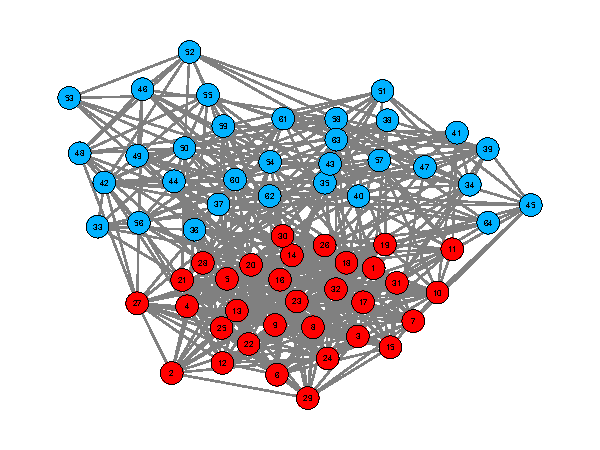
\includegraphics{curve-fitting-scratch_files/figure-latex/unnamed-chunk-2-1} \end{center}

\end{example}

If we observe the \(T_i\)'s, then we can use a standard polynomial
regression method to obtain \(\hat{\theta}\). Since we do not observe
them, the proposed iterative method is as follows:

\begin{enumerate}
\def\labelenumi{\arabic{enumi}.}
\tightlist
\item
  Initialize \(\hat{\theta}^{(0)}\) (e.g., randomly).
\item
  Estimate each \(\hat{t}_i^{(s)}\) by minimizing
  \(L(t_i, \hat{\theta}^{(s)} | x_i) = L_i = \|x_i - g(t_i | \hat{\theta}^{(s)})\|^2\).
\item
  Compute each
  \(\hat{x}_i^{(s)} = g(\hat{t}_i^{(s)} | \hat{\theta}^{(s)})\)
\item
  Estimate \(\hat{\theta}^{(s+1)}\) by minimizing
  \(L(\{\hat{t}_i^{(s)}\}, \theta | X) = \sum_i \|x_i - g(\hat{t}_i^{(s)} | \theta)\|^2\).
\item
  Repeat steps 2-4 until convergence.
\end{enumerate}

If we restrict \(g\) to be polynomials, then steps (2) and (4) have
closed-form solutions. Alternatively, we can estimate \(g\) using more
general forms, e.g., splines, which may require approximation.

\begin{example}

Write $g(t | \theta) = (g_1(t | \theta_1), ..., g_d(t | \theta_d))$ where $g_r(t | \theta_r)$ is the component of $g$ in the $r^{th}$ dimension and $\theta_r$ is the vector of parameters for the $r^{th}$ dimension. If $g_r$ are polynomials of degree $p$, then each $\theta_r$ contains up to $p + 1$ entries. 

Given the observed points $x_1, ..., x_n \in \mathbb{R}^d$ and their corresponding index points $t_1, ..., t_n \in \mathbb{R}$, we can find each $\hat{\theta}_r$ individually by $\hat{\theta}_r = A^{-1} b$ where $b \in \mathbb{R}^{p+1}$ and $b_k = \sum_i x_i t_i^k$ and $A \in \mathbb{R}^{(p+1) \times (p+1)}$ and $A_{kl} = \sum_i t^{(k-1) (l-1)}$.

On the other hand, if we have parameters $\theta$ but not the index points $t_i$, we can minimize each $t_i$ individually by finding the roots of a $p+1$ polynomial with coefficients that depend on $x_1, ..., x_n$ and $\theta$. 

In the following plot, we drew $n = 200$ points from the 2D H-W curve with $T_1, ..., T_n \stackrel{\mathrm{iid}}{\sim}Uniform(0, 1)$. 
The red line is the curve that was fit using the above method. 

\end{example}

\begin{center}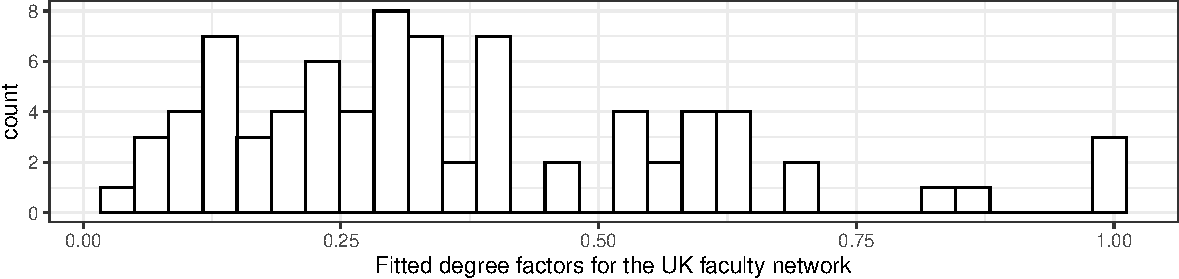
\includegraphics{curve-fitting-scratch_files/figure-latex/unnamed-chunk-3-1} \end{center}

One problem with this method is the parameterization of the curve is not
unique.

\hypertarget{estimation-with-noise}{%
\section{Estimation with Noise}\label{estimation-with-noise}}

\begin{example}

In the next example, we draw $A \sim \mathrm{RDPG}(X)$ using the same H-W curve and sample size as above and estimate the true latent positions (up to rotation). 

\end{example}

\begin{center}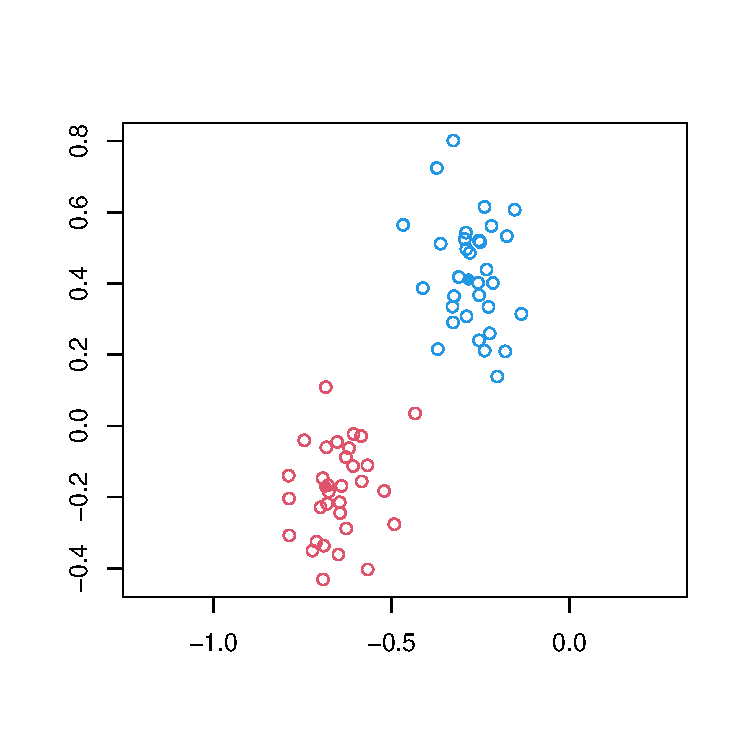
\includegraphics{curve-fitting-scratch_files/figure-latex/unnamed-chunk-5-1} \end{center}

\hypertarget{clustering}{%
\section{Clustering}\label{clustering}}

Next, suppose we have K curves parameterized by \(g^{(k)}\), with points
drawn along these curves. Then one possible clustering technique is as
follows:

\begin{enumerate}
\def\labelenumi{\arabic{enumi}.}
\tightlist
\item
  Assign an initial clustering (e.g., via spectral clustering).
\item
  Estimate the curve for each cluster.
\item
  Reassign the clusters by proximity to each curve.
\item
  Repeat 2 and 3 until convergence.
\end{enumerate}

\begin{example}

We again limit these to be quadratic functions in $\mathbb{R}^2$. 
Here, $K = 2$ and $n_1 = n_2 = 256$. 


\begin{center}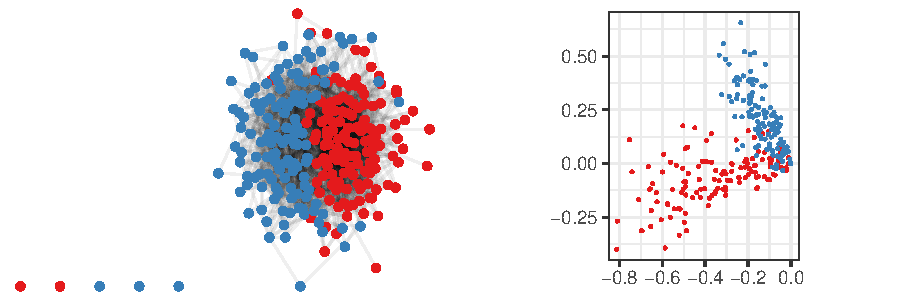
\includegraphics{curve-fitting-scratch_files/figure-latex/unnamed-chunk-6-1} \end{center}

Next, we draw $A \sim \mathrm{RDPG}(X)$ from the above example and apply the clustering and curve fitting to the ASE of $A$.
The community detection error in this example is 30\%.
In the following plot, the points are colored according to their true labels.


\begin{center}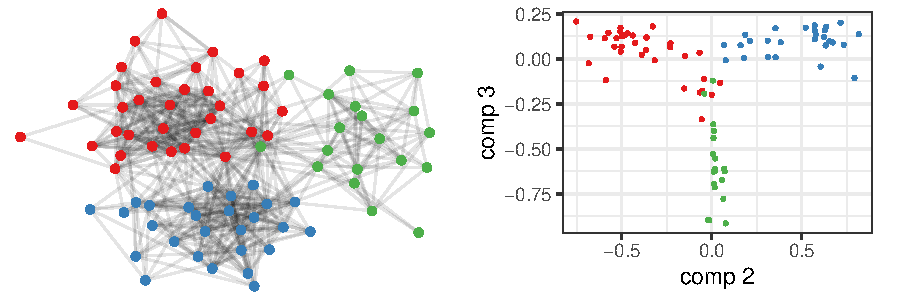
\includegraphics{curve-fitting-scratch_files/figure-latex/unnamed-chunk-7-1} \end{center}

\end{example}

A possibly more robust modification to this is to use Bezier curves for
\(g\). This is the same functional form as the polynomial curves we used
before, but with different basis functions. For the following examples,
we consider the quadratic Bezier curve, which has the following basis
form:

\[
g(t | p) = (1 - t)^2 p_0 + 2 t (1 - t) p_1 + t^2 p_2
\]

Where as before, \(g : [0, 1] \mapsto \mathbb{R}^d\) and
\(t \in [0, 1]\), and each \(p_r \in \mathbb{R}^d\). Thus if we can fit
each \(p_r\), then the procedure is the same as before.

Common methods for Bezier curve fitting do not require specification of
\(t_1, ..., t_n\). However, an ordering is required.

The curve fitting method is then modified as follows:

\begin{enumerate}
\def\labelenumi{\arabic{enumi}.}
\tightlist
\item
  Initialize \(\hat{p}^{(0)}\) (e.g., randomly).
\item
  Estimate each \(\hat{t}_i^{(s)}\) by minimizing
  \(L(t_i, \hat{p}^{(s)} | x_i) = L_i = \|x_i - g(t_i | \hat{p}^{(s)})\|^2\).
\item
  Reorder \(X\) according to \(t_1, ..., t_n\).
\item
  Estimate \(\hat{p}^{(s)}\) for the reordered \(X\) using Bezier curve
  fitting.
\item
  Repeat steps 2-4 until convergence.
\end{enumerate}

Then this becomes step 2 of the clustering method outlined above.

We can also estimate \(\hat{p} = (T^\top T)^{-1} T^\top X\) where
\(T = \begin{bmatrix} t_1 & \cdots & t_R \end{bmatrix}\) and each
\(t_r = \binom{R}{r} (1-t)^{R-r} t^r\), where \(R\) is the order of the
Bezier curve, so using the method for estimating \(t_1, ..., t_n\) as
described before, we can iteratively solve for \(\hat{p}\) in the same
manner. If we use soft clustering (e.g., EM as opposed to \(K\)-means),
we can also insert a diagonal matrix of weights \(W_k\) to obtain

\[\hat{p}_k = (T^\top W_k T)^{-1} T^\top W_k X\]

where \(X\) is the full data matrix, \(T\) is the full model matrix, and
\(W_k = w_k\) with the entries of \(w_k\) being the estimated
probability of each \(x_i\) being in cluster \(k\).

\begin{example}



We have two intersecting curves, $g_1(t) = \begin{bmatrix} t^2 & 2 t (1 - t) \end{bmatrix}^\top$ and $g_2(t) = \begin{bmatrix} 2 t (1 - t) & (1 - t) ^ 2 \end{bmatrix}^\top$. $n_1 = n_2 = 128$ points are drawn uniformly from each.


\begin{center}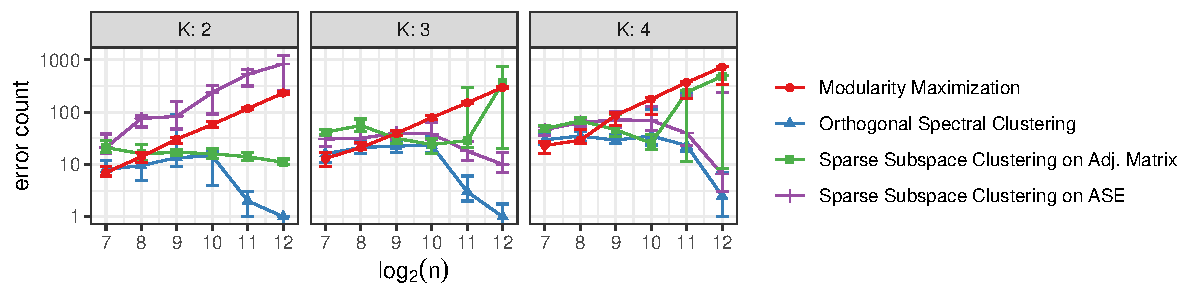
\includegraphics{curve-fitting-scratch_files/figure-latex/unnamed-chunk-9-1} \end{center}

We draw $A \sim \mathrm{RDPG}(X)$ and obtain the following ASE:


\begin{center}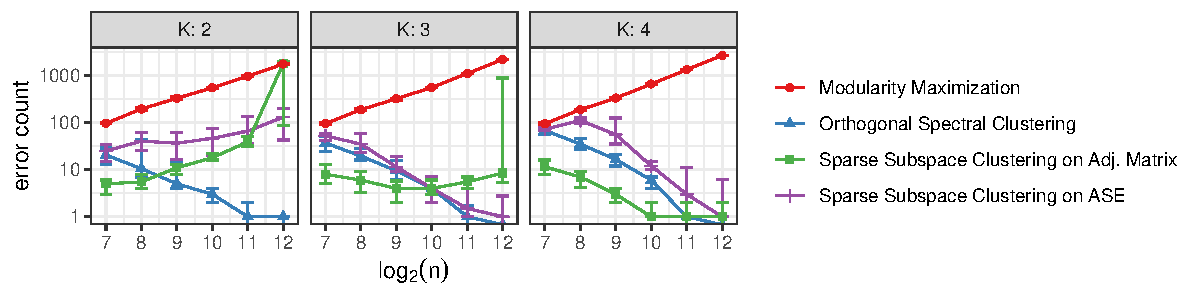
\includegraphics{curve-fitting-scratch_files/figure-latex/unnamed-chunk-10-1} \end{center}

Fitting two quadratic Bezier curves to these data yields a community detection error rate of 10\%. 
In the following plot, the points are labeled according to their estimated labels.


\begin{center}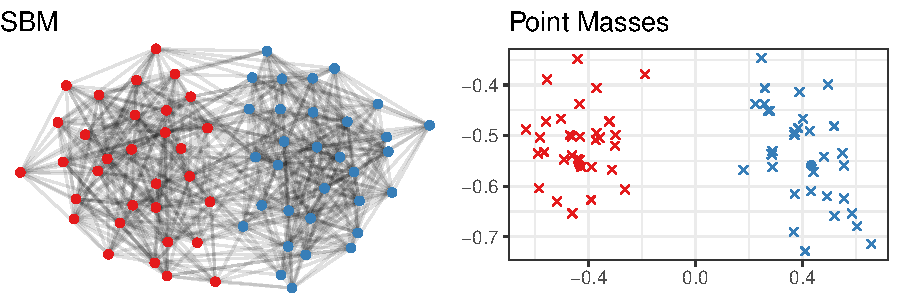
\includegraphics{curve-fitting-scratch_files/figure-latex/unnamed-chunk-11-1} \end{center}

\end{example}

  \bibliography{misc.bib}

\end{document}
